\chapter{Foundations in Chemistry}
	This part is all about understanding the basics. If you took triple science like me you should know the vast majority of this module.
	
\section{Fundamentals in chemical semantics 2.1.1}
	
	\paragraph{Isotopes} are atoms of the same element with different atomic masses.
	
	\paragraph{Atomic Structure} is, in this section, in reference to the number of protons neutrons and electrons found in an atom.
	Understanding that the Relative atomic mass of a proton is $\approx 1$ a neutron $\approx 1$ and an electron is negligible.
	OCR like questions which involve giving the repetitive isotopic mass of an element and ask you to calculate the number of neutrons o/e.
	
	\paragraph{Mass spectrometry} is a tool chemists use to identify the relative mass of ions.
	You need to be able to look at the readout from a mass spectrometer.
	
	First let us examine how a mass spectrometer works (you will see more of this).
	Fist we put a sample of the substance we are testing in the machine.
	The sample is vaporized and ionized to form positive ions.
	These positive ions are then accelerated and separate based upon the weight of the ion.
	The readout will give the mass-to-charge ratio on the x axis and relative abundance on the y.
	(there is a diagram in your book if I don't get round to making one.) The peaks represent isotopes if the substance is an element.
	
	In this section we use the percentage abundance\footnote{Derived from relative abundance} to work out a mean atomic mass.
	
	\paragraph{Relative atomic mass} is a term I have been using which has so far been left unexplained.
	I will clarify its meaning now. Relative atomic mass is the mass of an atom relative to $\frac{1}{12}$ the mass of \ch{^{12}C}.
	This term is almost identical to the terms relative isotopic mass, relative molecular mass and relative formula mass.
	$Mr$ is generally the algebraic identifier used and is the molar mass of a substance (which is in g mol$^{-1}$).
	In these notes if I say $Mr_{NaOH}$ I am referring to the Mr of Sodium Hydroxide.
	
	In case you have not managed guess it, to work out the relative formula mass one simply summates the atomic masses of the elements in the formula.
	The subscripts in formula mean x of this e.g. there are two chlorine atoms in \ch{C_2}.
	
\section{Basics in ionic compounds and equations 2.1.2}
	
	\paragraph{Shells} are a concept that, for now, you just need to accept.
	We will explore it further soon but just accept it for now.
	They contain electrons and want to be full.
	An atom with unfilled outer shell may loose an electron, or gain an electron from another atom. When this happens we call them ions. 
	
	The amount of electrons that an atom will loose/gain is fairly predictable.
	Looking only at the first three periods on the periodic table, the group numbers refer to the number of electrons the atom has in the unfilled outer shell.
	Group 0 has a full outer shell, group 7 has 7 electron in the outer shell, group 6 has 6 etc.
	
	Now given that there are a maximum of 8 electrons in the outer shell, and an atom wants to be stable, an element in group 7 is going to do the efficient thing and gain an electron, whilst an atom in group 1 is going to loose one.
	So take, for example Lithium and Chlorine. Lithium is in group one and will loose an electron.
	Chlorine is in group 7 so will gain an electron. If lithium gives an electron to chlorine it becomes \ch{Li+} and chlorine becomes \ch{Cl-}.
	Opposite charges attract and so we form an electrostatic bond between Lithium and Chlorine.
	We call this substance Lithium Chloride and this bonding mechanism is called \textit{Ionic Bonding}.
	To succinctly define ionic bonding would be as follows:
	
	 \begin{quote}
	 Ionic bonding is a bond formed by the electrostatic attraction between two oppositely charged ions.
	 \end{quote}
	 
	 \paragraph{Ions} are atoms or compounds with a charge.
	 There are some ions you need to remember, and remember there suffix too as it will help you name them.
	 \ch{NO3-} is the -nitrate ion, \ch{CO3^{2-}} is the -carbonate ion, \ch{SO4^{2-}} is the -sulfate ion, \ch{OH-} is the -hydroxide ion, \ch{NH4+} is the amonium- ion, \ch{Zn^{2+}} is the zinc- ion and \ch{Ag+} is the silver- ion.
	 The reason for all the - is that it makes creating the words easier.
	 For example, silver nitrate is \ch{AgNO3}.
	 The Positive ion then the negative one.
	
	\marginpar{\textbf{Hint} If the word has the suffix -ate, it means that oxygen is present in the ion}
	 
	 \paragraph{Equations} in chemistry refer to a system of expressing a chemical reaction. For example: \ch{2 NaOH + H2SO4 -> Na2SO4 + 2 H2O}.
	 As you can see we have the reactants on the right, products on the left and the big numbers balance the equation acting as the molar ratios for stoichiometry.
	 
\section{The mole}
	\paragraph{Moles} are a new way to look at measuring quantity.
	Instead of looking at how much of a substance we have by weighing it we can look at how much we have of a substance by looking at the number of particles we have of it.
	1 mole is equal to $6.02\times 10^{23}$ particles. This is all, usefully, designed around the gram. To show you what I mean take our good friend \ch{^{12}C}.
	If I get 1 mol of \ch{^{12}C} I will have 12 grams of it.
	This relationship works by design.
	So now we have the formula $m = nM_r$ where $n =$ number of moles and $m =$ mass.
	 
	\paragraph{Concentration} is a simple extension.
	Simply take the number of moles dissolved in a given volume of solvent then divide it by the volume.
	Concentration is measure it in mol dm$^{-3}$.
     
	\paragraph{A mole of gas} fills, in standard conditions (RTP), 24.0 dm$^3$ of space.
	The number of moles is directly proportional to the space filled.
	You can find this information on the formula sheet under ``Molar gas volume".
     
	When the substance isn't under standard conditions the ideal gas equation is used, $pV = nRT$. Lucky this is also sort of given.
	They give us a number called the ``Gas constant". This number gives us the units (J mol$^{-1}$ dm$^{-3}$).
	We know that pressure is measured in pascals, which have the S.I. unit N m$^{-2}$ and volume has the S.I. unit of m$^2$.
	So the product of volume and pressure is to be N m which is, as we all know, J.
	Using this mental gymnastics we can express the units like so, Pa m$^3$ mol$^{-1}$ K$^{-1}$. and we know this to be equal to 8.314.
	So the given (but hidden) formula is,
	\begin{equation}
		8.314 = \frac{pV}{nT}
	\end{equation}
	
	\paragraph{The Units} used in this calculation have no given conversions, The exam may well give $T$ in degrees centigrade and $p$ in atm. Here are some conversions:
    
	1 atm = 101 KPa (3 S.F)
	
	0  C = 273 K (3 S.F)
	
	\paragraph{Empirical formula} is the simplest whole number ratio of atoms of each element present in a compound.
	
	\paragraph{Molecular formula} the number and type of atoms of each element in a molecule.
    
    \paragraph{Determining formula} is a necessary part of this exam.
    They love questions along the lines of ``Raheem has found that his substance has a composition by mass of 70.00\% C, 6.67\% H and 53.33\% O. (a) work out the \textit{empirical formula} (b) given the Mr of the compound is 180, work out the \textit{molecular formula}."
    
    How is this to be approached?
    Well we have been given the \%age composition by mass.
    If we assume the \%age mass to be actual mass (given that we are working out a ratio) we can convert into moles.
    
    \[Mr_\textnormal{C} = 12.0\]
    \[Mr_\textnormal{H} = 1.0\]
    \[Mr_\textnormal{O} = 16.0\]
    \[\textnormal{Molar ratio (C:H:O)} = \frac{70.00}{12.0} : \frac{6.67}{1} : \frac{53.33}{16.0}\]
    \[\textnormal{Molar ratio (C:H:O)} = 3.33 : 6.67 : 3.33\]
    \[3.33 : 6.67 : 3.33 = 1 : 2 : 1\]
    
    Now we have an answer to part (a). \ch{CH2O}. To work out part (b) we need to set up an equation:
    
    \[n \times Mr_{\ch{CH2O}} = 180\]
    \[Mr_{\ch{CH2O}} = 30.0\]
    \[n = \frac{180}{30.0}\]
    \[n = 6\]
    \[6(\ch{CH2O}) = \ch{C6H12O6}\]
    
    \paragraph{Hydrated salts} are calculated in much the same way.
    They are expressed like this \ch{CuSO4.$n$H2O} and you will be given some numbers to workout $n$.
    Heating a substance removes the H2O making it anhydrous.
    To Hydrate simply devolve the salt in water and evaporate the water very slowly.
    
    \paragraph{Atom economy and \%age yield} are as simple as they sound.
    \%age yield is in reference to the percentage of the theoretical yield that was actually yielded.
    Atom economy simply refers to the number of waisted atoms (atoms that form waist products).
    Simply apply logic and understand these two concepts in terms of industry.
    
\section{Acids 2.1.4}

	\paragraph{The acids to remember} are the following:
	\begin{itemize}
		\item HCl is Hydrogen Chloride
		\item \ch{H2SO4} is Hydrogen Sulphate
		\item \ch{NOH3} is Nitric Acid
		\item \ch{KOH} is Potassium Hydroxide
		\item \ch{CH3COOH} is Ethanoic Acid (although it is commonly called Acetic Acid).
	\end{itemize}
	
	Acids release \ch{H+} ions when in aqueous solution.
	To examine the strength of an acid we must look at the dissociation of the \ch{H+} ions.
	Take for example HCl. The dissociation of HCl in aqueous solution looks like this, 
	\begin{center}
		\ch{HCl(aq) -> H^+(aq) + Cl^-(aq)} 
	\end{center}
	As you can see all of the hydrogen atoms have dissociated.
	This would make HCl a \textit{strong acid}. 
	
	Where the \ch{H+} ions only partially dissociate we call it a \textit{week acid}. Take Ethanoic acid, its dissociation in aqueous solution looks like this, 
	\begin{center}
		\ch{CH3COOH(aq) <=> H^+(aq) CH3OO^-(aq)}
	\end{center}
	 As we can see the \ch{H+} ions haven't entirely dissociated.
	 The \ch{<=>} implies that the reaction is incomplete and forms an equilibrium, So the acid hasn't completely dissociated.
	
	There is a point to be made that not all ionic compounds with hydrogen atoms are acids.
	It is only those compounds that form \ch{H+} ions when dissolved in aqueous solution that we call acids.
	
	\paragraph{The common bases} are metal oxides, metal hydroxides, metal carbonates and ammonia, \ch{NH4}.
	Bases neutralise an acid and form a salt.
	
	\paragraph{An Alkali} is a special type of base which, when dissolved in water, releases hydroxide ions.
	For example take the base \ch{Mg(OH)2},
	\begin{center}
		\ch{Mg(OH)2(s) + aq -> Mg^{2+}(aq) + 2 OH-(aq)}
	\end{center}
	We can see that \ch{Mg(OH)2} is an alkali as it releases \ch{OH-} ions when dissolved in aqueous solution.
	
	\paragraph{The alkali to remember} are the following:
	\begin{itemize}
		\item \ch{NaOH} is Sodium Hydroxide
		\item \ch{KOH} is Potassium Hydroxide
		\item \ch{NH3} is Ammonia
	\end{itemize}
	However you will be expected to know how to peace together bits you already know to construct your baces/alkali formula.
	
	\paragraph{You need to remember} that \ch{H+ + OH- -> H2O}, \ch{CO3^{2-} + 2 H+ -> H2O + CO2} and finally \ch{O^{2-} + 2 H+ -> H2O}.
	Using these ionic equations you should be able to form full equations.
	
	\paragraph{Titrations} are a piratical technique to achieve a neutralisation reaction.
	We take an acid and a alkali and we slowly add one to the other using a burette.
	This is a PAG and you probably will have done this.
	
	The preparation of a standard solution simply involves dissolving a exact and known mass of ionic compound and dissolving it in a know volume of water.
	This is done in a volumetric flask.
	
\section{Redox 2.1.5}

	\paragraph{OIL RIG} is a fantastic acronym.
	Oxidation Is Loss, Reduction is gain.
	Remembering this is vital.
	If we describe a reaction as having \textit{oxidised} X, we mean to say that X has lost electrons.
	If a reaction is described as having \textit{reduced} X, we mean to say that X has gained electrons.
	
	To write a redox reaction we have equations like this:
	\begin{center}
	\vspace{7mm}
	\ch{
		2 "\OX{o1, \ox[pos=top]{0,Na}}" + "\OX{r1, \ox[pos=top]{0,Cl}}" {}2
		->
		2 "\OX{o2,\ox[pos=top]{+1,Na}}" {}+ + 2 "\OX{r2, \ox[pos=top]{-1,Cl}}" {}-
	}
	\redox(o1,o2){\small OX: $- 2\el$}
	\redox(r1,r2)[][-1]{\small RED: $+ 2\el$}
	\vspace{7mm}
	\end{center}
	We use Roman numerals to indicate oxidation numbers, memorise the following oxidation numbers:
	\begin{itemize}
		\item Oxygen has the oxidation number -2 unless in peroxide, in which case it is -1
		\item Hydrogen has the oxidation number +1 unless in a metal hydride in which case it is -1
		\item Fluorine has the oxidation number -1
	\end{itemize}
	So to work out whether a chemical has been oxidised or reduced we do the following.
	
	\begin{enumerate}
		\item Find the balanced symbol equation,
		
		\ch{2 Al + 3 H2SO4 -> Al2(SO4)3 + 6 H2}
		
		\item Then we fill in the oxidation numbers for the ones we know,
		
		 \ch{2 "\ox{0, Al}" {} + 3 "\ox{+2, H}" {}2 "\ox{-2, SO}" {}4 -> Al2 "\ox{-6,(SO}" {}4)3 + 6 "\ox{0, H}" {}2}
		 
		\item The \ch{Al2 "\ox{-6,(SO)3}" {}4} has no overall charge so the oxidation numbers must add to 0,
		
		\ch{"\ox{+6, Al}" {}2 "\ox{-6,(SO)3}" {}4}
		
		\item Now we have \ox{+6, Al}$_2$ we can see that \ox{+3, Al}. So Aluminium went from Al to \ox{+3, Al} meaning it has been oxidised in this reaction.
		
		\item The hydrogen went from \ox{+2, H}$_2$ to \ch{H2}. This is a reduction so we say hydrogen has been reduced.
	\end{enumerate}
	
	A faster way to instantly know is to look at the oxygen.
	We can see that Hydrogen has lost oxygen in this reaction while Aluminium has gained oxygen.
	By looking at it this way we can very quickly see what has been reduced and what has been oxidised.
	
	In summary oxidation numbers refer to the number of electrons individual atoms in compounds have lost/gained.
	They are like charge but apply to atoms and not the overall compound.
	They are used to explain whether a reaction has oxidised an atom or reduced it.
	
\section{Electron structure 2.2.1}

	\paragraph{Shells} are areas where there is a heigh probability of finding an electron.
	They are split by looking at major energy levels.
	The period an atom is in indicates how many shells it has.
	The number of electrons that can fit into a shell can be worked out by $2n^2$ where $n$ is the shell number.
	
	\paragraph{Shells are sub-divided} into sub-shells. The ones you need to know are as follows,
	\begin{itemize}
		\item s orbital which can hold 2 electrons, one in all shells
		\item p orbital which can hold 6 electrons, one in all but shell 1
		\item d orbital which can hold 10 electrons, one in all but shells 1 \& 2
	\end{itemize}
	They fill in order.
	
	\paragraph{Orbitals} are regions around the nucleus which can hold up to two electrons, both have opposite spin.
	This diagram is of a P orbital and the arrows indicate the spin,

	\begin{center}
		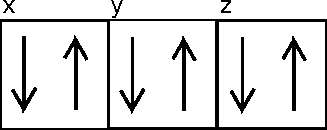
\includegraphics{Porbital}

	\end{center}
	This is a Full P orbital and as you can see, each sub-orbital (denoted by the box) contains two electrons of opposite spin.
	They don't, however, fill sequentially. It take less energy to fill like this,

	\begin{center}
		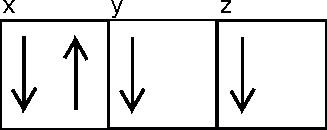
\includegraphics{P4orbital}
	\end{center}

	X get the first, Y gets the second Z gets the third and X gets the last.
	All the orbitals work in a similar way and the number of sub-orbitals can be found by dividing the maximum electron capacity by 2.
	
	\paragraph{Order of fill} is as follows, 1s$^2$2s$^2$2p$^6$3s$^2$3p$^6$4s$^2$3d$^{10}$4p$^6$ in the standard format $x$s$^n$ where $x$ is the shell and $n$ is the number of electrons in the shell.
	
	The examination may well ask you to write the electron configuration of an atom.
	Unless otherwise instructed, a short cut is to use a noble gas as a base.
	For example if I said write the electron configuration of sodium you can say [Ne]3s$^1$.
	You need to know how to do this for all elements upto and including Kr
	
	\paragraph{Energy levels} are the reason different shells fill differently.
	As we go up the shells we also ascend in energy level.
	The most interesting part is the 4s sub-shell and the 3d sub-shell.
	The 4s sub-shell and the 3s sub-shell have very similar energy levels.
	The 4s sub-shell is, however, slightly lower so the 4s fills first.
	When the 3d sub-shell fills the energy level falls meaning, the 4s fills before 3d and the 4s empties before 3d.
	This is important when looking at the electron configuration of D Block ions.
	
\section{Bonding 2.2.2}

	\paragraph{Ionic bonding} is the first of the two types of bonding I need to cover.
	As mentioned before,
	\begin{quote}
		Ionic bonding is a bond formed by the electrostatic attraction between two oppositely charged ions.
	\end{quote}
	We have cations, which are positively charged ions, and anions, which are negativity charged ions. When the cation and the anion meet they form a ionic bond. It is, as you guessed, the bonding which holds together ionic compounds like NaCl.
	 
	\paragraph{Dot-and-cross diagrams} are the same as they have always been.
	Used for drawing the simplest of ionic bonds, that of metal - non-metal.
	Just remember the square brackets, the outer shell is drawn and the charge goes at the top right of the brackets. %(potential for diagram if I have time)
	 
	\paragraph{Giant ionic lattices} are the result of ionic bonding. This is what gives ionic compounds their crystalline structure.
	Take sodium chloride, each \ch{Na+} ion is surrounded by 6 \ch{Cl-} ions and vis-versa, they are strongly attracted in all directions.
	This gives it a cubic structure and is why table salt breaks into small cubes. 
	 
	\paragraph{Ionic bonds physical properties} are fairly obvious. The strong electrostatic forces within a giant ionic lattice require high energy to break.
	This makes ionic compounds almost always \textit{solid} at room temperature and mean that they have a \textit{high} boiling point.
	 
	Ionic compounds will usually dissolve in polar solvents, such as water.
	The polar molecules in the solvent break down the lattice creating dissociated ions, which are then surrounded by the solvent.
	However some ionic compounds will not be very soluble.
	This is because the electrostatic attraction between the ions may be too strong for a polar solvent, such as water, to break down.
	In general the greater the ionic charge, the less soluble the ionic compound will be.
	 
	Electrical conductivity in a solid ionic compound is zero. This is because the ions are not free to move around.
	However if the compound is dissolved or melted it will be able to conduct electricity.
	This is because the ionic bonds have been broken down and the ions are free to carry charge (mobile charge carriers).
	 
	\begin{itemize}
		\item Have heigh melting and boiling points
		\item Tend to dissolve in polar solvents
		\item Only conduct electricity when in liquid state or dissolved in aqueous solution.
	\end{itemize}
	 
	\paragraph{Covalent bonding} , to quote the specification, is ``the strong electrostatic attraction between a shared pair of electrons and the nuclei of the bonded atoms."
	\begin{itemize}
	 	\item Non-metallic elements such as \ch{H2} and \ch{O2} form covalent bonds.
	 	\item Non-metallic compounds such as \ch{H2C} and \ch{CO2} form covalent bonds.
	 	\item Even polyatomic ions are covalently bonded such as \ch{NH4^+}
	\end{itemize}
	
	\paragraph{Dot and Cross} diagrams are very similar to the dot and cross diagrams for ionic bonding.
	Instead of drawing them septate in there own square brackets we simply draw them as overlapping circles with dots and crosses for the various electrons.
	
	There are the following three types of covalent bonding that you are expected to know about,
	\begin{enumerate}
		\item Single covalent bonding, this is where there is one shared pair of electrons per nuclei.
		\item Multiple covalent bonding, this is where there are multiple pairs of shared electrons per nuclei
		\item Dative covalent bonding, this is where the shared pair is supplied by only one of the atoms.
	\end{enumerate}
	You will be expected to draw dot-and-cross diagrams with atoms of up to six electron pairs, including lone pairs.
	This means the bonding seen in \ch{SF6} will roughly be the most complicated.
	
	\ch{NH4^+} is a good example of a dative covalent bond. A \ch{H+} ion meets amonia and amonia provides the electron pair for the covalent bond.
	
	\paragraph{Average Bond Enthalpy} is simply a measure of the average amount of energy required to break say a \ch{Br-Br} bond.
	This acts as an indicator to the bonds strengthen, the larger the value of the average bond enthalpy, the stronger the covalent bond.
	
\section{The shapes of simple molecules and ions 2.2.2}
	
	\paragraph{You need to know} the shapes of, and bonding angles in, molecules and ions with up to six electron pairs (including lone pairs) surrounding the central atom as predicted by electron pair repulsion.
	
	\paragraph{Electron pair repulsion} is a modal used for explaining and predicting shapes of covalently bonded molecules.
	It works on the principle that electron pairs, you guessed it, repel. They arrange themselves around an atom as wide apart as possible.
	They do this in 3D, which may sound obvious, but so far in chemistry we have worked only with 2D models.
	To draw 3D diagrams we need to understand the following standards,
	\begin{itemize}
		\item \chemfig{A-B} is used for a bond in the same plane as the paper
		\item \chemfig{A<B} is used for a bond coming out of the paper
		\item \chemfig{A<:B} is for bonds going into the plane of the paper
	\end{itemize}
	
	\paragraph{Bonded pair/lone pair} repulsion is stronger than bonded pair/bonded pair.
	This is because the lone pair of electrons occupying more space than the bonded pair, overall resulting in a slightly higher repulsion from the lone pair.
	The bonding angle is, therefore, reduced by around 2.5\degree for every lone pair.
	
	\paragraph{Common, and basic examples} are molecules such as, \ch{CH4} which has a bonding angle of 109.5\degree and no loan pairs and forms a tetrahedral structure; \ch{NH3} which has a bonding angle of 107\degree with one lone pair and this is pyramidal; finally \ch{H2O} which is non-linear and with its two lone pairs has a bonding angle of 104.5\degree .
	
	The last shapes to be familiar with are trigonal planar which have a bonding angle of 120\degree , linear which are 180\degree and octahedral which are 90\degree . (I may add diagrams if I get time but page 71-72 of the textbook has good ones.)
	
\section{Electronegativity and bond polarity 2.2.2}
	\paragraph{The Pauling scale} is a scale used to measure the electronegativity of an atom. As we go right, across the periodic table, the electronegative increases along side a decrease in atomic radius. As we move up the table we see an decrease in the number of shells, hence a decrease in atomic radius, so we see then an increase in electronegativity. So the nearer F in the table, the higher the electronegitivity.
	
	\paragraph{Electronegitivity} simply refers to the amount of attraction a atom in a covalent bond has over the shared pair of electrons in a covalent bond.
	
	\paragraph{Polar bonds} are covalent bonds between two elements with different electronegitivities.
	\chemfig{H^{\delta +}-Cl^{\delta -}} is an example of a polar bond, and by extension a polar molecule.
	H has a lower electronegativity than chlorine causing the chlorine in the covalent bond to become slightly negative.
	This type of bonding is called a permanent dipole.

	\paragraph{Covalent, Polar covalent and ionic} are defined here by the difference in electronegitivity of the bonding atoms.
	Where the difference is zero we call the bond covalent.
	Where it is less than 1.8 we call it polar covalent and where it is greater than 1.8 we call it ionic.
	
	\paragraph{Larger molecules} are interesting in the sense that a we need to look at structure to see if the overall molecule is polar or non-polar.
	Take \ch{H2O}, this has a non-liner structure. Both the \chemfig{H^{\delta +}-O^{\delta -}} bonds are polar and given its non-liner structure, these polar bonds don't cancel out.
	This makes \ch{H2O} a polar molecule because it has an overall dipole.
	
	However, take \ch{CO2}, a similar covalent molecule with two \chemfig{C^{\delta +}=O^{\delta -}} polar bonds.
	But this is where it changes. The structure is liner.
	This means that the two bonds cancel out \chemfig{O^{\delta -}=C^{\delta +}=O^{\delta -}}.
	Meaning that the overall molecule, in the case of \ch{CO2}, is non-polar.
	
\section{Intermolecular Forces 2.2.2}
An important distinction from ionic or covalent bonding is that these are forces between separate molecules.

	\paragraph{Permanent dipole - dipole interactions} are caused by polar molecules attracting each other and forming a permanent electrostatic interaction.
	This is very similar to giant ionic lattices but occurs with polar covalent molecules such as water.
	The distinction is that it is between separate molecules.
	
	Generally permanent dipole interactions are conducive to a higher boiling point, given the extra energy required to break the interaction.
	
	\paragraph{Hydrogen bonding} is ``intermolecular bonding between molecules containing N, O or F and the H atom of –NH, –OH or HF". It is a special type of permanent dipole-dipole interaction. 
	
	Hydrogen bonding has a significant influence on the properties of many molecules.
	Water, for example, is affected by hydrogen bonding.
	Hydrogen bonding allows for the formation of a more open lattice structure by holding the molecules apart.
	The result is that ice is less dense than liquid water.
	
	\paragraph{London Forces} are temporary dipole-dipole interactions.
	Electrons move, and as such may cause a molecule to be temporarily polar.
	This temporary polarity may allow the formation of an instantaneous dipole.
	This, on a micro scale, isn't a long lasting, however when we look on a macro scale with a massive number of molecules this has a large affect.
	This interaction occurs in every molecule.
	
	London forces strength is dependant on the number of electrons.
	Elements with large number of electrons have stronger London forces due to the greater probability of an interaction.
	So as we move down the periodic table we would expect a higher boiling point (where london forces are the primary interaction).
	
	\paragraph{Simple molecular lattices} are formed when a simple molecular substance
	\footnote{A simple molecular substance is one with a defined number of atoms and with definite formula} are in there solid form.
	They are simply put ``covalently bonded molecules attracted by intermolecular forces, e.g. \ch{I2}, ice".
	The molecules in simple covalent lattice are held together by repetitively \textit{week} intermolecular forces, The atoms within the molecules are held together by very \textit{strong} covalent bonds.
	
	\paragraph{Solubility} of these different types of compounds follow this basic rule, in general: Polar compounds will be soluble in polar solvents and non-polar compounds will be soluble in non-polar solvents.
	
	The reason for the polar compounds being soluble in polar solvents is that the polar solvent attracts the polar compound.
	This attraction, in a similar way to ionic compounds, acts to pull apart the permanent dipole-dipole bonds and causing the compound to dissolve.
	
	The reason for the non-polar compounds dissolving in non-polar solvents is much the same.
	The intermolecular interactions are the same so the solvent is able to break down the simple covalent lattice.
	
	\paragraph{Electrical conductivity} is nil for simple covalent structures.
	There are no mobile charged particles meaning that there will be no way for the substance to be conductive.